\documentclass[a4paper,12pt]{report}

\usepackage[utf8]{inputenc}      
\usepackage[T1]{fontenc}        
\usepackage[french]{babel}       
\usepackage{graphicx}           
\usepackage[colorlinks=true, linkcolor=blue, urlcolor=blue]{hyperref}
\usepackage{xurl}            
\usepackage{amsmath, amssymb}   
\usepackage{geometry}            
\usepackage{fancyhdr}
\usepackage{float}       

\geometry{
  a4paper,
  top=3cm,
  bottom=3cm,
  left=4cm,
  right=4cm
}
\setlength{\headheight}{40pt}
\pagestyle{fancy}
\fancyhf{}
\fancyhead[L]{
    \small
    \textbf{Loris DROUHOT} \\
    BUT Informatique
    
}
\fancyfoot[C]{\thepage}

\title{Rapport de Stage}
\author{Loris DROUHOT}
\date{\today}

\begin{document}

\maketitle
\newpage
\thispagestyle{empty}

\chapter*{Remerciements}
\addcontentsline{toc}{chapter}{Remerciements}

Je souhaite remercier M. François LALAY, développeur web full-stack, qui fut maître de stage pendant ces 10 semaines, pour sa patience, sa confiance mais surtout sa pédagogie. Apprendre à ses côtés fut un réel plaisir. Il a su me guider afin de progresser sans pour autant tout m'expliquer à chaque fois, ce qui m’a forcé à rechercher par moi-même afin d’obtenir des réponses à mes questions techniques.

\vspace{1em}

Je tiens aussi à remercier M. Ronan MÉVELLEC, Directeur, qui a pris le temps, une après-midi, dans son programme chargé, de me rencontrer afin que l’on puisse échanger sur ma situation, le stage, ainsi que de m’expliquer précisément ce qu'est l’ATD 16.

\vspace{1em}

Je remercie aussi l’ensemble de l’équipe de l’ATD 16 qui m’a très bien accueilli, pris le temps de m’écouter lors de réunions, mais aussi de m’expliquer leur travail, ce qui fut très enrichissant. Plus précisément l'équipe projet Numérobis : Lionel CLERCQ, Responsable du pôle numérique, Charlotte CIARDULLI et Perrine MADIOT, toutes deux chargées du support administration numérique et logiciels métiers, ainsi que Pierre SAUZE, expert en numérique, pour leur temps et leurs conseils lors des réunions hebdomadaires du projet de développement.

\vspace{1em}

Enfin, je remercie aussi mon professeur référent, M. Sébastien FAUCOU.

\newpage
\chapter*{Résumé}
\addcontentsline{toc}{chapter}{Résumé}
\thispagestyle{empty}

Dans le cadre de ma formation de Bachelor Universitaire Technologique deuxième année à l’Institut Universitaire Technologique de Nantes, j’ai réalisé un stage de 10 semaines au sein de l’Agence Technique du Département de la Charente. Lors de ce stage, j’ai mis en pratique ainsi que développé mes connaissances et compétences en développement web. J’ai donc développé une nouvelle fonctionnalité intégrée à l'application interne de l’agence. Il s'agit d'une page de simulation permettant à un agent de l'ATD 16 de calculer le prix qu’aurait à payer un adhérent pour les politiques auxquelles il souhaite souscrire en rentrant les variables nécessaires (nombre d’habitants, voirie, etc.).


As part of my second-year Technological University Bachelor’s program at the Institut Universitaire Technologique de Nantes, I completed a 10-week internship within the Agence Technique du Département de la Charente. During this internship, I put into practice and developed my knowledge and skills in web development. I have therefore developed a new feature integrated into the agency’s internal application, it is a simulation page allowing an agent from ATD 16 to calculate the price that a member would have to pay for the policies they wish to join by entering the necessary variables. (number of inhabitants, roads, etc.).

\tableofcontents               

\newpage
\thispagestyle{empty}
\vspace*{\fill}            
\begin{center}             
Tous les mots suivis d'un astérisque sont définis dans le glossaire
\end{center}
\vspace*{\fill}            


\chapter{Introduction}         
Étudiant en deuxième année de BUT Informatique, je dois réaliser un stage en entreprise d'une durée de 10 semaines afin de valider mon année. Ce stage se déroule entre le 22 avril 2025 et le 27 juin 2025, le but de ce stage est de mettre en pratique les compétences acquises dans notre cursus, ainsi que de nous faire découvrir le monde professionnel en informatique.

\vspace{1em}

J'ai eu la chance de pouvoir réaliser mon stage à l'Agence Technique Départementale de la Charente (ATD 16), j'ai donc été intégré à son pôle numérique en compagnie de François LALAY, mon maître de stage, unique développeur de l'application de l'agence, ainsi qu'à l'équipe projet Numérobis. A mon arrivée j'ai réalisé un mini-projet avec les technologies utilisées pour le développement de l'application de l'agence, afin de me familiariser avec. Ces technologies sont le framework \footnote{Un framework c'est une infrastructure logicielle qui offre un cadre pour le développement}* React Next.js pour le front-end\footnote{Le front-end c'est la partie avec laquelle le client peut interagir du code}*, et le framework* PHP Symfony ainsi que API platform pour le back-end\footnote{Le back-end c'est la partie du logiciel qui accède aux données et les traite}*. Une fois ce mini-projet terminé, j'ai pu commencer ma première mission, qui était le développement de la fonctionnalité de simulation sur l'application web interne à l'agence, et donc développer aussi bien la partie front-end* que back-end*.

\vspace{1em}

Afin de réaliser cette mission de la meilleure manière et le plus efficacement possible, j'ai donc tout d'abord pris connaissance de la grille tarifaire et de ses contraintes: on m'a demandé de réaliser moi-même un cahier des charges fonctionnel et des wireframes, à partir des premières informations et besoins. Lors des réunions hebdomadaires avec l'équipe projet Numérobis, j'ai présenté ce cahier des charges fonctionnel, on m'a alors précisé l'étendue de la mission et exprimé de nouveaux besoins. Une fois le cadrage délimité, j'ai pu commencer le développement du simulateur. Le projet Numérobis suit un cycle de développement agile (méthode de travail nécessitant des réuinions quotidiennes), 
mais avec des réunions seulement deux fois par semaine du fait que François LALAY est le seul développeur, mais il souhaitait garder un contact avec les utilisateurs.

\vspace{1em}

Dans le but de compléter la mission qui m'a été confiée, j'ai utilisé de nombreux outils, allant de la connaissance théorique aux documentations des différents langages de programmation. Le concept le plus important quand j'ai travaillé sur la partie back-end* de ma mission a été la sérialisation et donc aussi la désérialisation, ce sont les processus centraux du fonctionnement d'une API* Rest. Ce sont eux qui assurent que les données soient converties au bon format pour l'envoi, puis convertissent les données reçues au format du langage utilisé. Ces concepts sont intégrés à Symfony et API Platform nativement, il suffit de bien les utiliser. Il m'a aussi fallu me pencher sur d'autres concepts plus spécifiques aux outils utilisés, comme le type verbe\footnote{Les verbes HTTP sont GET, POST, PUT et DELETE} HTTP de la route API, les différents événements attachés à ces routes. Pour la partie front-end*, la théorie est moins présente car les données et l'application sont spécifiques, j'ai donc été amené à utiliser des outils propres aux frameworks* avec lesquels on travaille, comme les hooks React ou les stores Zustand.

\vspace{1em}

Pour trouver des solutions à la plupart de mes problèmes, un type d'outil est primordial : les documentations. Quand elles sont bien renseignées, les documentations ont souvent la réponse à tous nos problèmes généraux pour un langage ou un framework*. Lorsque j'avais des problèmes plus précis, alors les forums ou les IA sont aussi des outils intéressants, même s'ils ont des limites naturelles posées par le fait qu'ils ne connaissent pas notre projet. Il s'agit alors de trouver un cas général donnant une idée de la solution à notre problème.

\vspace{1em}

Dans un premier temps, je présenterai l'agence, son statut spécifique, son fonctionnement, ainsi que son intérêt pour les services publics charentais.


Dans une seconde partie, je parlerai des outils qui m'ont été utiles, la réalisation de ma mission de développement principale, ainsi que d'autres petites missions

\chapter{Développement}

\section{L'Agence Technique Départementale de la Charente}
L'Agence Technique Départementale de la Charente est un service public. Fondée en 2014, elle regroupait déjà les compétences de l'AMO (Assistance à Maîtrise d'Ouvrage) et du juridique, puis a intégré les compétences du SDITEC (numérique et cartographique) en 2018. L'agence propose un nombre conséquent de compétences permettant d'aider, de conseiller ou d'assister les différentes collectivités territoriales de Charente. Pour l'organigramme structurel voir annexe


M. Ronan MÉVELLEC, directeur et fondateur, explique cela comme une mutualisation des moyens des collectivités, chaque collectivité n'a pas forcément les moyens de payer des agents pouvant réaliser tout genre de tâches, qu'elles soient numériques, juridiques ou cartographiques. C'est là où l'ATD 16 prend tout son intérêt, elle permet de centraliser toutes compétences (Aménagement, Numérique, Juridique et Cartographique) au sein d'un seul service public, auquel les collectivités peuvent demander de l'aide, à condition d'adhérer aux politiques adéquates.

\subsection{Fonctionnement économique}

Étant un service publique, l'argent injecté et récolté est surveillé de près, c'est pourquoi il y a un Conseil d'Administration, présidé par M. Michel CARTERET, ce conseil prend les décisions pour l'ATD, qu'elles soient budgétaires, salariales ou toutes autres choses. Ce conseil est composé de représentants des adhérents à l'ATD 16. Monsieur le directeur ne peut qu'appliquer les décisions du conseil, néanmoins la plupart des idées sont suggérées par l'ATD puis validées par le conseil.

L'ATD 16 fonctionne sur un modèle de volets principaux, d'adhésions optionnelles et d'appuis ponctuels. En premier lieu, l'ATD propose deux volets principaux, le volet AMO, incluant l'assistance à maîtrise d'ouvrage et l'assistance juridique, et le volet Numérique, incluant la maintenance du parc informatique, l'administration numérique, un système de convocations électroniques et un profil acheteur sur les marchés publics. Une fois adhérents à l'un ou les deux volets, les collectivités ont le droit de souscrire aux adhésions optionnelles, comptant par exemple l'entretien de la voirie, le RGPD, un parcours cybersécurité, l'assistance sur logiciels métiers, ou encore la mise à disposition de logiciels de cartographie permettant plein de choses comme la gestion des cimetières par exemple. Un adhérent peut cumuler autant d'adhésions optionnelles qu'il le souhaite, le prix des volets et des adhésions optionnelles est calculé en général au nombre d'habitants. Il existe d'autres variables comme le nombre de boîtes de messagerie pour l'adhésion aux "boîtes de messagerie" ou encore la voirie pour l'entretien des routes. Pour les détails de la grille tarifaire voire annexe.

Enfin, l'ATD propose aussi des appuis ponctuels : services rendus irrégulièrement sur demande d'une collectivité ; il peut s'agir de suivi d'opérations après la mise en route d'un projet par l'AMO, de prêt de matériel, ou encore d'adressage pour les communes. Il existe plusieurs types de collectivités territoriales pouvant accéder aux services de l'ATD 16, la majorité sont des communes, mais il y a aussi des communautés de communes, des syndicats ou encore le département lui-même.



\subsection{Environnement de Travail}

En ce qui concerne l'environnement de travail, chaque pôle de l'agence possède son bureau sur le site de la Combe à Angoulême, Charente. Je travaille sur un HP ProBook 450 G7, les 8 Go de RAM sont insuffisants afin de faire tourner le serveur de l'application web et de l'API* pour le développement, mais je m'en sors plutôt bien, j'ai en plus deux écrans iiyama. Pour ce qui est du software, on m'a laissé le choix de l'IDE, j'ai choisi Visual Studio Code, c'est adapté au PC pas très performant que j'avais. Quelques extensions comme le visualiseur de base de données sont nécessaires afin de limiter le nombre d'outils. Afin de tester les routes API, j'ai utilisé Postman, logiciel permettant, entre autres, de faire des requêtes API. Mariadb est utilisé pour avoir une copie de la base de données de production en local. Pour la gestion de projet j'ai utilisé le tableau Kanban\footnote{C'est un tableau utilisant la méthode Kanban qui organise sont travail tâche par tâche} de Jira.

\section{Les outils}
Au cours du stage, j'ai utilisé et découvert de nombreux outils, que je connaissais et utilisait déjà comme Git et GitLab, ou de nouveaux comme Jira pour faire de la gestion de projet. Cependant, les outils que j'ai le plus utilisés de loin, ce sont les documentations des langages et technologies utilisés.

\subsection{Git}
Git est certainement le software le plus important dans le monde de l'informatique avec Linux. C'est un gestionnaire de versions, c'est-à-dire qu'il permet de stocker un ensemble de fichiers, d'y apporter des modifications et de conserver ainsi l'historique de ces modifications. Ici, je n'ai pas découvert Git, mais son utilisation dans le monde professionnel, la logique de "production" et de "développement" et donc le fonctionnement des branches. Avant ce stage, mon utilisation de Git était assez rudimentaire, je me contentais de la simple branche "main", puis j'ai ajouté mes modifications une fois que cela fonctionnait en local.


Grâce à ce projet, mon utilisation a évolué, le dépôt contenant l'API* et l'application possède deux branches majeures "main" et "develop", ces deux branches sont protégées. Pour développer, je crée une nouvelle branche à partir de develop, puis commit des modifications au fur et à mesure. Une fois satisfait de mon code je le push sur la branche distante, et enfin crée une "merge request" afin que François LALAY puisse voir mes modifications et les accepter dans la branche develop. Puis une fois qu'il juge les avancées satisfaisantes, il merge la branche develop avec la branche main avant de passer au déploiement, ceci est donc le workflow\footnote{Le workflow c'est une suite de tâches} de développement.

\subsection{Gestion de Projet}
Le développement de ce simulateur étant mon plus gros et surtout long projet à ce jour, je ne pouvais pas négliger la gestion du projet, même si je développais seul dessus. Lors de mon arrivée, j'ai réalisé un cahier des charges fonctionnel, qui devait présenter ma vision du projet, que j'ai partagé lors de ma première réunion hebdomadaire avec l'équipe proejt Numérobis. Effectivement, deux fois par semaine, le lundi puis le jeudi, il y a des réunions avec l'équipe projet Numérobis, composée de :
\begin{itemize}
    \item Lionel CLERCQ, Responsable du pôle numérique
    \item Charlotte CIARDULLI, chargée du support administration numérique et logiciels métiers
    \item Perrine MADIOT, chargée du support administration numérique et logiciels métiers
    \item Pierre SAUZE, expert en numérique
\end{itemize}
François LALAY y présente ses avancées sur le projet Numérobis, j'ai donc aussi pris part à ces réunions sur ma période de présence, où je présentais donc les évolutions du simulateur. 


Lors de ces réunions, chacun peut donner ses impressions et proposer des changements ou ajouts, et donc afin de ne pas me perdre dans les demandes, j'ai utilisé Jira et son tableau Kanban, où je place dans la colonne "TO DO" les tâches à développer, "IN PROGRESS" la tâche en cours et dans "DONE" les tâches terminées.

\begin{figure}[H]
    \centering
    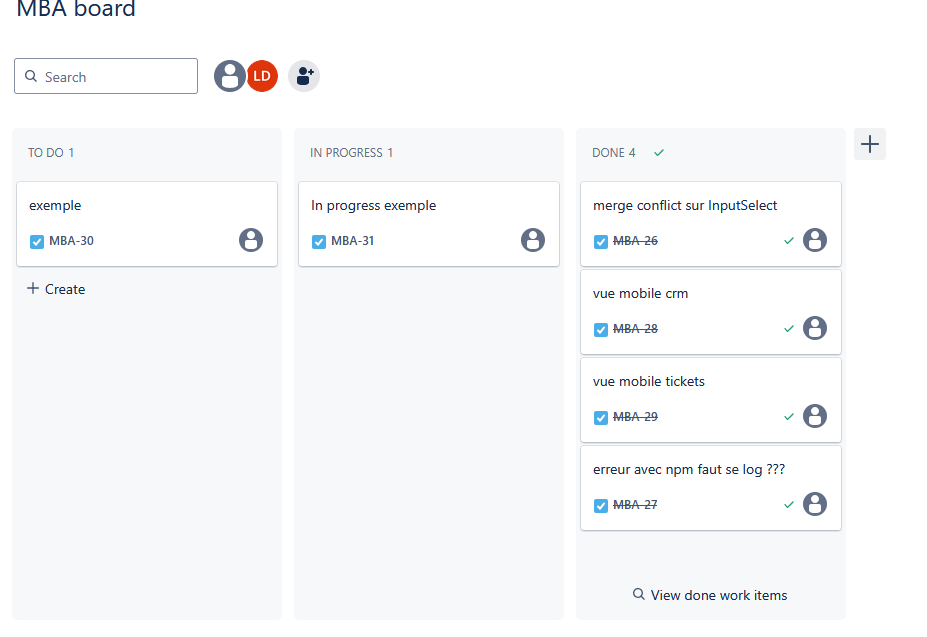
\includegraphics[width=0.8\textwidth]{kanban.png}
    \caption{Tableau Kanban de Jira}
    \label{fig:kanban-jira}
\end{figure}

\subsection{Les documentations et l'IA}
Certainement le type d'outils que j'ai le plus utilisé, je les ai bien longtemps ignorés, durant mon cursus, au profit d'outils plus "performants", notamment l'IA, mais lors de mon stage je me suis rendu compte de leur intérêt. Documentation d'API Platform, Tailwind CSS, MDN, autant de documentation que de langages et technologies utilisés. Une fois que j'ai compris comment les utiliser, elles se sont avérées être des outils très puissants. J'ai eu, cependant, quelques soucis avec la documentation Symfony, dont je trouve que la recherche n'est pas très précise, et qui manque parfois d'explications et d'exemples. Ces différentes documentations qui sont à la base de mon projet, ont répondu à nombre de mes questionnements et recherches.

Un autre outil m'a aussi parfois aidé, Chat GPT, que j'ai beaucoup utilisé pendant le BUT, j'ai donc voulu faire l'effort de moins l'utiliser pendant le stage, ce que j'ai réussi. De plus, il a montré très vite ses limites, car s'il est effectivement très performant pour aider dans des petits projets universitaires, ici la masse conséquente de contexte le limite dans l'exactitude de ses réponses. Je l'ai donc utilisé dans deux types de cas :
\begin{enumerate}
    \item quand je ne savais absolument pas comment faire quelque chose, même pas l'idée de comment le faire, j'ai alors utilisé l'IA afin d'avoir un exemple pour commencer.
    \item quand j'avais besoin d'explications dont je ne trouvais pas la réponse dans la documentation.
\end{enumerate}
 

\section{Le simulateur}
\subsubsection{L'application Numérobis}
L'application interne de l'ATD 16, Numérobis, est un ERP (Enterprise Resource Planning), le choix du développement d'une application web interne a été conditionné par la complexité du système tarifaire de l'ATD.

\subsection{Explication de la mission}

La mission principale de mon stage est donc la réalisation d'un simulateur de prix d'adhésions sur l'application Numérobis, site interne à l'ATD 16. Ce simulateur doit pouvoir donner un prix pour une structure adhérente, en tenant compte des variables renseignées. Une simulation existait déjà, mais elle se limitait à une seule nouvelle adhésion et ne prenait en compte que les variables déjà rentrées. Cette nouvelle version doit dépasser ces limites, il faut pouvoir calculer une ou plusieurs nouvelles adhésions pour une structure déjà adhérente mais aussi pouvoir simuler une adhésion d'une nouvelle structure. 

Il y a cependant plusieurs contraintes :
\begin{enumerate}
    \item La surcotisation du multi-site doit donner seulement la valeur de la surcotisation (pas le total)
    \item L'exception de réduction de prix du parcours cybersécurité quand il y a une souscription au RGPD
    \item Le simulateur doit être utilisable sur mobile
\end{enumerate}

En résumé, il faut une page permettant de :
\begin{enumerate}
    \item Simuler une nouvelle adhésion en partant de zéro
    \item Simuler une nouvelle adhésion en utilisant une structure déjà existante
\end{enumerate}

\subsection{Le Back-end}
Le back-end* de l'application web est une API* Rest, développée avec Symfony et API platform. Afin de développer le simulateur, j'ai dû comprendre la logique des entités Symfony, les relations entre elles ainsi que le fonctionnement des routes API platform. Cette période de compréhension du projet a été grandement accélérée par le fait qu'au 3ème semestre j'avais réalisé une application web en utilisant Symfony pour la SAE. J'étais donc déjà familier avec le fonctionnement de beaucoup d'aspects, comme les entités, les contrôleurs et Doctrine\footnote{Outil facilitant la gestion de la base de données, grace au concept d'ORM (Object Relational Mapping) ca permet de ne pas écrire de SQL} mais aussi plus globalement avec le langage PHP en lui-même.

Cependant, il fallait que je comprenne le fonctionnement d'API platform, c'est un framework* PHP basé sur Symfony, l'application développée au 3ème semestre n'utilisait pas d'API, tout était fait dans le même projet, back et front. API platform permet de créer des API* REST avec Symfony. En créant les routes classiques automatiquement (GET, GET Collection, PUT, POST, DELETE), on peut aussi attacher des événements à ces routes comme "validate". Ce sont des services Symfony, ce qui va faire qu'un objet arrivant par cette route POST va être regardé afin de savoir s'il correspond aux contraintes de la base de données. De plus, API platform utilise le format Hydra JSON, ce qui permet de mieux comprendre ce qui est envoyé mais aussi de plus simplement retrouver des objets avec l'IRI (Internationalized Resource Identifier), c'est le champ "@id" dans "hydra:member".

\begin{figure}[ht]
    \centering
    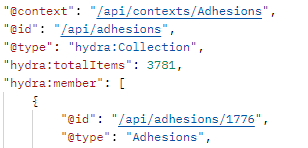
\includegraphics[scale=0.8]{hydraJSON.png}
    \caption{Exemple de hydra JSON}
    \label{fig:hyda-json}
\end{figure}

\subsection{Le controller simulateur}
Afin de réaliser le back-end* du simulateur, je me suis grandement inspiré de la route de simulation déjà existante. En premier lieu j'ai analysé les paramètres nécessaires au calcul, puis j'ai créé des groupes de dénormalisation, c'est en fait une annotation qui permet de dire à l'API* les données attendues pour la route POST. Ensuite, la fonction de calcul des prix a besoin de trois paramètres, une structure, une adhésion et une année, il faut donc que le json envoyé dans le body de la requête contienne les éléments nécessaires à la création de ces trois objets.

\begin{figure}[H]
    \centering
    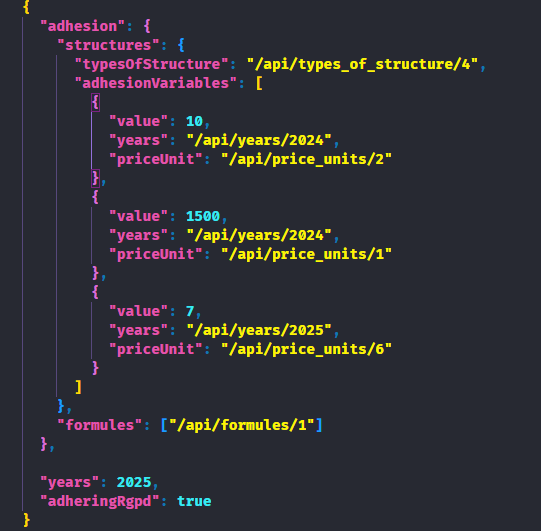
\includegraphics[scale=0.6]{jsonSimu.png}
    \caption{Exemple de json pour le simulateur}
    \label{fig:json-simu}
\end{figure}

On remarque donc ici que la Structure est imbriquée dans l'Adhésion, ces deux objets sont donc créés à la dénormalisation quand l'objet arrive avec la requête, on retrouve aussi dans ce json tous les champs du groupe de dénormalisation, et qui suffisent donc à créer les deux objets. L'objet Année est un objet qui existe déjà en base de données, on transmet donc ici seulement l'année, qui va nous permettre, grâce aux repository de Symfony, de récupérer l'objet Years correspondant. Voici un graphique expliquant les principes de sérialisation et déserialisation.

\begin{figure}[H]
    \centering
    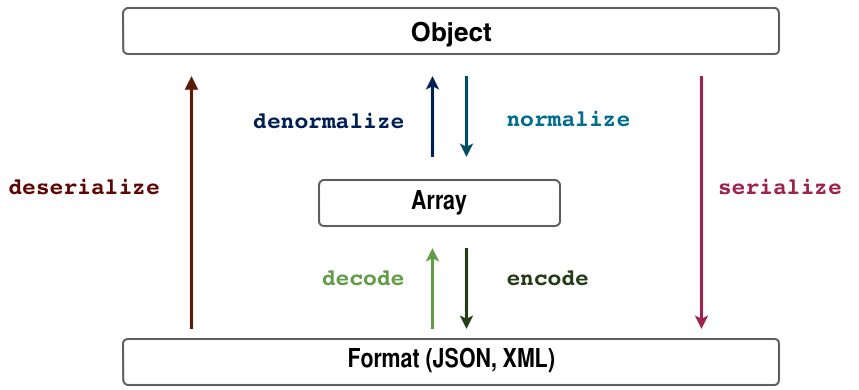
\includegraphics[width=0.8\textwidth]{SerializerWorkflow.png}
    \caption{La serialization}
    \label{fig:serialization}
\end{figure}

Ensuite, il y a deux exceptions majeures dans le calcul :
\begin{itemize}
    \item La politique de maintenance de parc informatique multi-site est une augmentation de 25\% du prix du volet numérique, il faut donc en plus de la formule multi-site, les formules du volet numérique, puis calculer leur prix, puis recalculer avec le multi-site afin d'obtenir le prix d'augmentation causé par le multi-site.
    \item La deuxième arrive dans le cadre de la politique "Parcours cybersécurité", si l'adhérent adhère déjà à la politique RGPD alors le prix de la politique est réduit de 30\% supplémentaire, et donc pour gérer cette exception, le json possède un champ "adheringRgpd", qui donne l'information sur si cette structure adhère ou pas au RGPD. si c'est le cas, alors le controller ajoute la formule de RGPD avant le calcul, grâce au repository de Symfony, afin que la formule de calcul le prenne en compte
\end{itemize} 
Afin de toujours avoir l'information sur l'ID des formules problématiques, leur ID est stocké dans un fichier .ENV, qui n'est pas sauvegardé sur Git, mais qui évite ces "nombres magiques". Il y a juste à changer l'ID dans le fichier .ENV et tous les endroits où c'est importé récupèrent alors le nouvel ID.

\subsubsection{Documentation}

API platform supporte nativement le format de documentation d'openAPI* (anciennement Swagger), et donc cela crée une documentation à l'adresse \href{https://dev.API.numerobis.atd16.fr/API}{adresse-API/API}. Sur cette page, on retrouve donc la documentation de toutes les routes de l'API, avec une documentation par défaut pour les routes standards. Cependant ma route n'est pas standard, et donc pour la documenter correctement, j'ai utilisé des DTO (Data Transfer Object). J'ai donc créé deux DTO, un "input" (entrée) et "output" (sortie). Grâce au groupe de dénormalisation et au DTO, la documentation décrit parfaitement ce qui est nécessaire dans le body de la requête. Ces DTO décrivent donc ce qui est attendu en entrée et en sortie de la route.

\begin{figure}[ht]
    \centering
    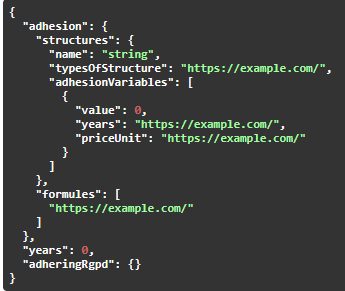
\includegraphics[scale=0.8]{docSimulatorInput.png}
    \caption{Documentation de la route API}
    \label{fig:swagger-simulator-in}
\end{figure}


\subsubsection{Tests}
Ayant écrit du code dans l'API, il faut bien évidemment le tester. J'ai donc créé une batterie de tests assurant une couverture de cas. Ce sont des tests fonctionnels, c'est-à-dire que l'on va tester le fonctionnement de l'API, afin de savoir si elle renvoie les bonnes valeurs ou bien les erreurs dans les cas échéants. Dans les tests déjà écrits dans le projet, François LALAY utilise Zenstruck, qui permet de générer facilement des objets aléatoires pour le testing, mais aussi de réinitialiser la base de test entre chaque test, je l'ai donc aussi utilisé. J'ai donc testé mon contrôleur en lançant aussi la totalité des tests afin de vérifier si mes modifications n'ont pas cassé quelque chose autre part dans le code.

\subsection{Le Front-End}

\subsubsection{Fonctionnement de React}
React est tout d'abord une librairie Javascript, elle fonctionne sur le modèle d'un arbre, chaque composant possède des enfants qui peuvent être d'autres composants React ou bien du JSX (c'est le code qui ressemble à du HTML dans le retour des composants). L'affichage de ces composants s'appelle le rendu, quand un composant se rend, ca veut dire qu'il s'affiche à nouveau avec de nouvelles valeurs si besoin. Dans les composants rendus côté client, on peut utiliser des "hooks" react, ce sont des fonctions qui permettent de stocker des états ou encore d'utiliser le cycle de vie des composants. Par exemple "useState", ce hook permet de garder une valeur entre les différents cycles de vie, et donc chaque fois que cet état est mis à jour, le composant se rend à nouveau, ainsi que tous ses enfants. Afin d'optimiser les performances de l'application web, il faut viser le minimum de rendu possible.

\subsubsection{Le simulateur}

Le simulateur se découpe en cinq zones majeures : un header, la liste des adhésions, le détail de l'adhésion sélectionné, l'importation d'une structure ainsi que les variables d'adhésions.

\vspace{1em}

Le header est plutôt simple, il contient le prix total des adhésions, simulé et importé s'il y a, ainsi que le sélecteur de type de structure. Sélectionner un type de structure est nécessaire pour le calcul.

\vspace{1em}

La liste des adhésions, c'est l'endroit où on affiche la liste qui contient les données envoyées à l'API. On retrouve dans cette liste toutes les données importantes relatives aux adhésions dans le simulateur : le titre de la politique, le prix simulé, ainsi que les formules. Le nom de chaque politique est cliquable pour afficher le détail des formules et pouvoir décocher ou cocher celles que l'on veut. Sur le côté gauche, on retrouve un groupe de boutons  : le premier (ajouter), ouvre une modale qui permet de choisir une politique à ajouter, le deuxième supprime la politique courante et le dernier efface toute la liste. Les composants affichés sont inspirés de composants déjà développés par François LALAY, que j'ai modifiés afin de faire apparaître les informations voulues.

\begin{figure}[H]
    \centering
    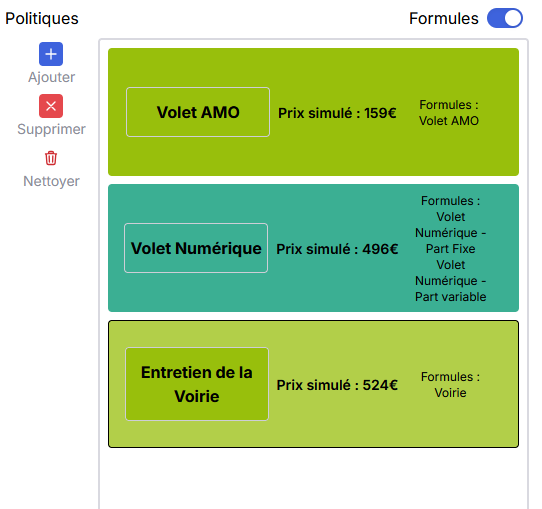
\includegraphics[scale=0.5]{adhesionList.png}
    \caption{Liste des adhésions}
    \label{fig:list-adhe}
\end{figure}

\vspace{1em}

Le composant de détail consiste essentiellement en un groupe de checkbox pour choisir les formules. À l'origine, les formules étaient récupérées par un appel API, mais par souci d'optimisation, j'injecte désormais dans le composant les formules à afficher, ce qui réduit le nombre d'appels à l'API. Ce composant apparaît aussi dans une modale quand on sélectionne une nouvelle politique, ce qui permet de faire disparaître l'affichage classique de ce composant pour la vue mobile.

\begin{figure}[H]
    \centering
    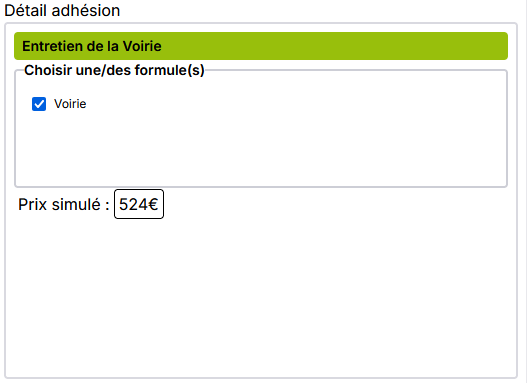
\includegraphics[scale=0.6]{detailAdhe.png}
    \caption{Détail adhésion}
    \label{fig:detail-adhe}
\end{figure}

Le composant d'import ne comporte visuellement qu'une seule chose, la barre de recherche de structure. Une fois qu'on sélectionne une structure, on récupère les données avec l'API, puis je les traite afin de correspondre au format nécessaire à l'affichage et au calcul de la simulation. Une fois la structure importée, on affiche ses adhésions ainsi que ses variables connues. De la même manière que pour le détail d'adhésion, ce composant disparaît en vue mobile et s'affiche dans une modale quand on clique sur le bouton "importer" (présenté plus tard avec la vue mobile).

\begin{figure}[H]
    \centering
    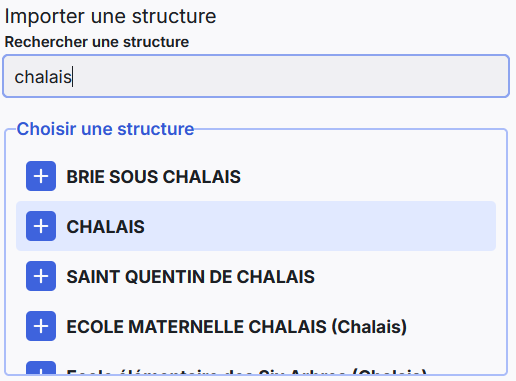
\includegraphics[scale=0.6]{import.png}
    \caption{L'importation de structures}
    \label{fig:import-struc}
\end{figure}

Ce composant est une liste d'"input contrôlés", un input contrôlé en React, c'est un input où l'on va stocker sa valeur à chaque modification, pas de bouton de validation, ça permet de tout le temps connaître la valeur de l'input. Ici, c'est une liste d'input contrôlés, c'est-à-dire qu'avec un seul "useState" on garde la trace de toutes les variables. La liste de variables est quant à elle récupérée par un appel API* au chargement de la page.

\begin{figure}[H]
    \centering
    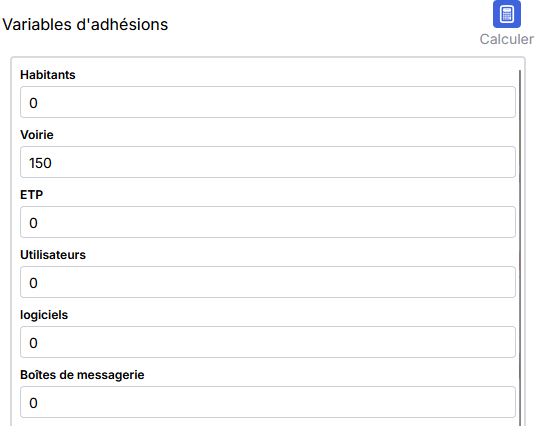
\includegraphics[scale=0.4]{adheVar.png}
    \caption{Les variables d'adhésion}
    \label{fig:adhe-var}
\end{figure}

Comme expliqué précédemment, la vue mobile faisait partie des demandes dès le début du développement. La question de la vue mobile tombe plutôt dans le domaine du CSS que du React, même si quelques changements ont été nécessaires de ce côté, comme la création des deux modales de détail et d'import. Après avoir discuté avec mon maître de stage du design mobile, il m'a fait remarquer que dans la plupart des applications, notamment de scroll comme TikTok et Instagram réels, ont les actions placées sur le côté droit et en bas, les zones d'accessibilité du pouce.

Tailwind CSS utilise un système de breakpoints\footnote{Ce sont points de rupture défini pour adapter le design d’un site aux différentes tailles d’écran}, par exemple avec le tag "md:" précédent une classe, celle-ci devient effective qu'à partir d'un affichage d'une largeur minimum de 768 pixels. Comme expliqué dans la documentation de Tailwind, ces paliers s'activent quand l'écran est supérieur à la largeur, il faut donc comprendre que l'affichage mobile doit être développé en premier, car on changera le comportement avec les marqueurs pour les écrans plus grands. Cependant, l'application Numérobis n'a pas été développée pour le mobile, et moi-même, m'y étant intéressé qu'une fois le simulateur fonctionnel, j'ai dû réécrire les classes Tailwind avec en configuration par défaut le mobile, et l'affichage bureau derrière des tags "md:". Ici, on a un contenant flex, avec une disposition en colonne pour la vue mobile (flex-col) puis en ligne si affichage plus large (md:flex-row).


\begin{verbatim}
<div className="flex H-full flex-col gap-2 md:flex-row">
    <p> Hello <p>
    <p> World <p>
</div>
\end{verbatim}


J'ai donc transformé les boutons d'actions à gauche de la liste d'adhésions en une barre d'actions qui reste en bas de l'écran, et ajouté un bouton "importer" qui permet d'afficher une modale avec le composant d'import de structure. J'ai aussi inversé l'affichage des prix et du nom dans la liste des adhésions afin d'avoir la zone cliquable à droite.

\begin{figure}[H]
    \centering
    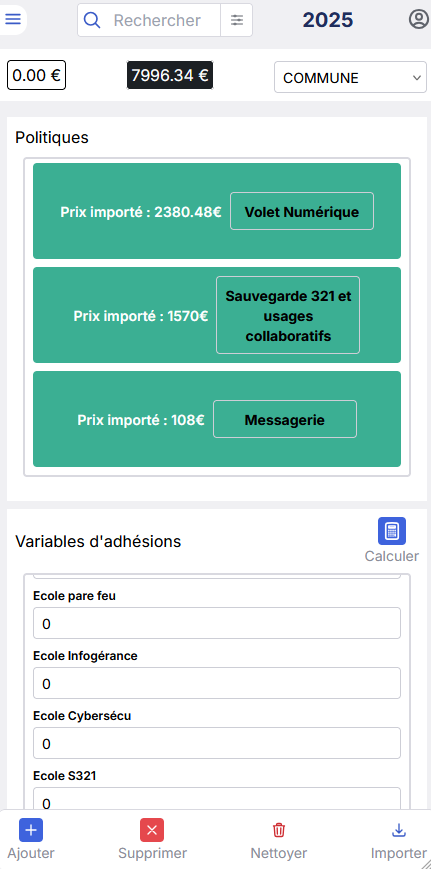
\includegraphics[scale=0.4]{vueMobile.png}
    \caption{Vue mobile}
    \label{fig:mobile-view}
\end{figure}


\section{Refactoring* avec Zustand}
Dans la première version du simulateur, j'ai utilisé les contextes de React pour pouvoir transmettre des informations en profondeur dans l'arbre React et aussi pour les modifier. Les contextes permettent d'éviter de faire des cascades de props\footnote{Les props sont des données transmises à un composant React depuis son parent}.

\begin{figure}[H]
    \centering
    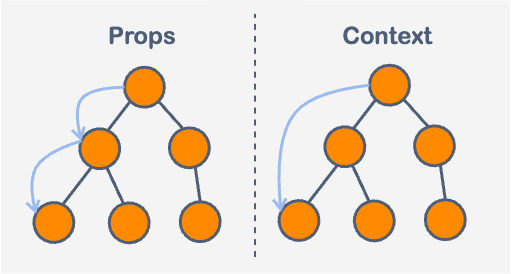
\includegraphics[scale=0.4]{props+vs+context.png}
    \caption{Contextes React}
    \label{fig:context-react}
\end{figure}

Ils fonctionnent sur le principe suivant : dans un composant parent, on crée un contexte et un état avec "useState".Puis dans le "return" du composant, on crée un "Provider" du contexte avec en valeur soit seulement l'état, soit l'état et sa méthode de modification si l'on a besoin de le modifier.

Dans le simulateur, j'ai eu besoin de transmettre beaucoup d'informations dans les composants, je me suis donc très vite retrouvé avec beaucoup de contextes et de providers dans la section de ma page. Ce qui rend, d'une, le code très peu lisible, car tous les états sont créés dans ce composant et de deux un souci d'optimisation. Comme expliqué précédemment, lorsqu'un état change, le composant se rend à nouveau ainsi que tous ses enfants. Combinez ça avec plusieurs contextes qui peuvent être modifiés et on obtient une page qui se rend entièrement à chaque modification.

\begin{figure}[H]
    \centering
    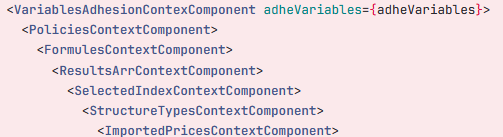
\includegraphics[scale=0.6]{providerHell.png}
    \caption{Le "Provider Hell"}
    \label{fig:provider-hell}
\end{figure}

Dans un premier temps, j'avais déplacé la création des états et des contextes dans des composants à part, afin d'améliorer la lisibilité, mais cela ne règle pas les problèmes d'optimisation. Mon tuteur, François LALAY, m'a orienté vers une librairie qu'il utilise dans l'application Numérobis, Zustand. Zustand est une librairie de state management pour React, ça permet de créer un "store", qui va stocker les données que l'on veut partager entre différents composants. Ce store est indépendant de React, les composants vont donc pouvoir interagir avec, afin récupérer les infos nécessaires. De plus, grâce aux sélecteurs de Zustand, seulement sont mis à jour les composants qui utilisent une valeur du store qui a été modifiée, ce qui réduit grandement le nombre de rendus. On retrouve donc dans ce store les données stockées ainsi que les méthodes de modification, cependant, tout comme les états React, les valeurs sont immutables, c'est-à-dire qu'on va "remplacer" par la nouvelle valeur, plutôt que de modifier l'ancienne.

\begin{figure}[H]
    \centering
    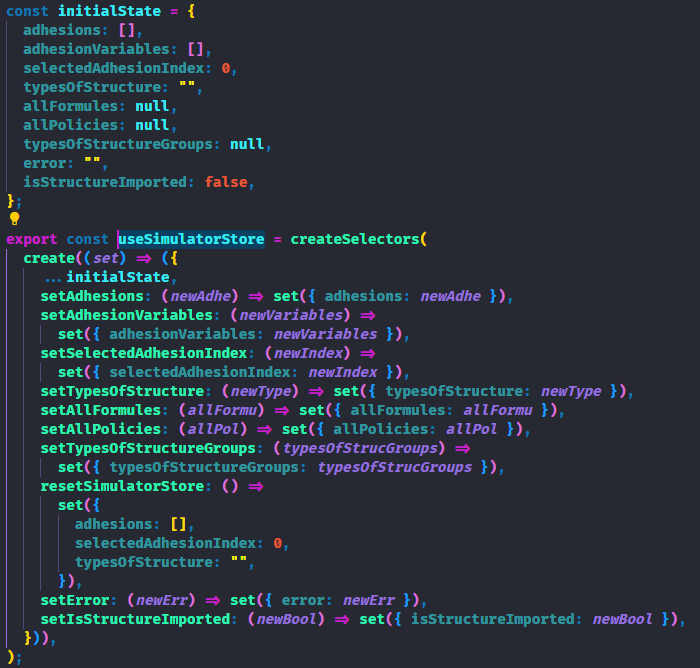
\includegraphics[scale=0.4]{storeZustand.png}
    \caption{Mon store Zustand}
    \label{fig:store-zustand}
\end{figure}

Le deuxième point important que m'a permis de faire Zustand, c'est la refactorisation de mon code. Du fait d'avoir déplacé les données de mon composant section au store, j'ai pu mieux isoler les logiques de chaque composant. Le fait de tout traiter dans la section m'avait contraint à y centraliser la logique. Maintenant, la logique est séparée et donc plus lisible et compréhensible pour chaque composant. Par exemple, à la fin du développement de la première version, donc avec les contextes et sans aucun refactoring, le fichier de la section de la page a atteint environ 350 lignes de codes, maintenant ce fichier ne fait que 21 lignes, car plus aucune logique ne s'y trouve, j'y organise simplement la disposition de la page.

\section{Autres petites missions}
Ayant terminé ma mission principale plutôt rapidement, j'ai réalisé d'autres petites missions. La première fut de développer une vue mobile utile pour la globalité de l'application web. Une première contrainte était que je ne pouvais pas modifier la vue bureau, et donc seulement la vue mobile. De plus Numérobis n'a pas été pensé pour une utilisation sur téléphone. J'ai donc commencé par adapter le layout principal, ce layout toujours présent est en deux parties, une barre de navigation latérale et un header. Évidemment, ce type de layout n'est pas adapté à une vue mobile. J'ai donc utilisé les breakpoints Tailwind, j'ai fait le choix d'intégrer la barre de navigation dans un popover, élément s'affichant au-dessus du contenu, qui s'affiche en cliquant sur un bouton ajouté au header.

\begin{figure}[H]
    \centering
    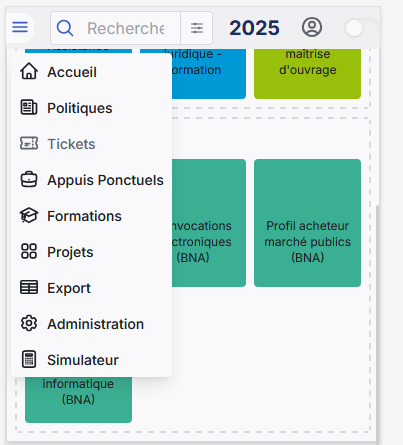
\includegraphics[scale=0.6]{headerMob.png}
    \caption{Header mobile}
    \label{fig:header-mob}
\end{figure}

Afin de toujours avoir le header accessible en vue mobile j'ai utilisé la position "sticky", c'est-à-dire que l'élément est dans le flux normal du document, mais si l'on scroll, le header devient fixe en haut de la fenêtre. Cela permet de garder le header en haut de page dans la vue bureau, mais aussi de toujours l'avoir en haut de l'écran quand on scroll sur mobile. J'ai aussi dû réduire le nombre d'informations comparé au header de la vue bureau afin que tout loge dans la largeur d'un mobile.

J'ai ensuite adapté la disposition des différentes pages en mobile, de manière à ce qu'elles soient consultables. 

\vspace{1em}

Ma deuxième mission secondaire a été l'implémentation d'un mode sombre. Tailwind le permet facilement à l'aide du tag "dark:". Ce tag active la classe derrière les deux points, quand la classe "dark" se trouve plus haut dans l'arbre HTML, c'est le même fonctionnement que pour le design responsive. Cependant, cette méthode nécessite d'écrire explicitement chaque changement du mode sombre dans tous les composants. Cela est faisable en cours de développement mais terriblement long sur un projet où ça n'a pas été fait. J'ai donc fait des recherches afin de trouver une solution, le fichier de configuration de Tailwind est le fichier où l'on va pouvir enregistré par exemple les couleurs que l'on va utilisé dans l'application. François LALAY a choisis sa palette de couleur avec Radix UI, site qui propose des progressions de couleurs qui ont été étudié afin d'optimiser l'accessibilité, critère absolument vital pour un site car cela fait partis des choses regardées par google pour le référencement du site. Ces progressions comportent une dizaine de couleurs, partant des couleurs de fond jusqu'aux couleurs de textes. Radix Ui donne aussi la version mode sombre de chaque gamme, facilitant son développement.

\begin{figure}[H]
    \centering
    
\includegraphics[scale=0.4]{colorRadixUi.png}
    \caption{Exemple de couleurs de Radix UI}
    \label{fig:radix-colors}
\end{figure}

Après quelques recherches, j'ai trouvé la solution. Il faut définir des variables de couleurs CSS dans le globals.css. Je crée donc le thème classique ainsi que le thème sombre, et dans chacun je rentre toutes les couleurs correspondantes avec le même nom pour les équivalences. C'est-à-dire que la couleur primary-200 par exemple se définit avec le code \#e1e9ff pour le thème classique, mais avec le code \#1d2e62 pour le thème sombre. Ce qui permet donc de ne pas avoir à réécrire les couleurs dans chaque composant. Quand on est sur le thème classique toutes les variables de couleurs prennent une certaine valeur, qui change quand on passe au thème sombre.

\begin{figure}[H]
    \centering
    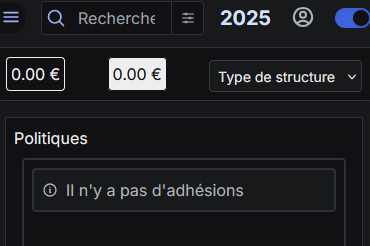
\includegraphics[scale=0.5]{exempleDarkmode.png}
    \caption{Le mode sombre de Numérobis}
    \label{fig:dark-mode}
\end{figure}

Une fois cette solution implémentée j'ai découvert un autre problème, Tailwind permet de modifier l'opacité de la couleur d'un composant simplement avec un "/50" à la suite de la couleur. Par exemple, cette annotation dit que l'opacité de la couleur est à 50\%. Ce système fonctionne avec Tailwind car les couleurs du framework sont au format rgba (Red Green Blue Alpha), l'Alpha définit l'opacité, cependant dans mon implémentation des thèmes les couleurs sont en hexadécimal. Il a donc fallu convertir toutes les couleurs de hexadécimal à RGB, puis dans la config Tailwind ajouter "/ <alpha-value>" pour expliciter qu'on attend une valeur d'opacité (mise à 1 (100\%) par défaut). Grâce à ce changement on peut donc utiliser les annotations d'opacité.

\begin{verbatim}
primary: {
        50: "rgb(var(--color-primary-50) / <alpha-value>)",
}
\end{verbatim}

\chapter{Conclusion}

Ce stage de 10 semaines à l'Agence Technique de la Charente m'aura permis d'avoir une expérience intéressante et surtout enrichissante, sur le plan professionnel principalement, car même si le penchant technique est très formateur, c'est surtout sur le plan professionnel que je pense avoir le plus progressé. Que ce soit la communication avec les utilisateurs, la gestion de projet, les réunions, c'est le genre de choses dont on a du mal à évaluer l'importance en tant qu'étudiant.

\vspace{1em}

Sur le plan technique, le fait de m'être obligé à moins utiliser l'IA m'a fait progresser dans la réflexion sur la résolution de problèmes. De plus, l'utilisation de nouvelles technologies m'a appris à utiliser plus efficacement les documentations, ainsi qu'à comprendre les outils par moi-même. François LALAY fut aussi un excellent formateur, il a su me guider afin que je progresse et découvre la plupart des solutions par moi-même.

\vspace{1em}

Le développement du simulateur fut un projet très enrichissant pour moi. Le fait de toucher au back-end* aussi bien qu'au front-end* me permet de mieux comprendre l'architecture d'une application fonctionnant avec une API* Rest. Mais aussi, de par la complexité de la grille tarifaire et le fait que ce soit un projet qui va être utilisé et non universitaire, j'ai dû apprendre à comprendre les demandes des clients/utilisateurs de l'application web et donc m'adapter à ce qu'ils veulent.

Ce projet fut très formateur et enrichissant. Le fait de développer en front-end ainsi qu'en back-end m'a permis de mieux comprendre le fonctionnement d'un site web qui utilise une API. J'ajouterai que le fait de développer un projet qui va être utilisé oblige à se confronter aux utilisateurs et de comprendre leurs besoins.

\vspace{1em}

Je suis conscient que le simulateur est perfectible, mais je suis cependant très fier de ce projet, mon plus long à ce jour. Je suis arrivé en n'ayant pas un grand affect pour le développemnt web, mais ce stage m'a fait changer d'opinion.

\chapter{Sources}
Toutes les sources en lignes ont été consultées en Juin 2025

\begin{enumerate}
    \item Documentation PHP : \url{https://www.php.net/manual/en/}
    \item Documentation Symfony : \url{https://symfony.com/doc/current/index.html}
    \item Documentation API platform Symfony : \url{https://API platform.com/docs/symfony/}
    \item Documentation Doctrine : \url{https://www.doctrine-project.org/projects/doctrine-orm/en/3.3/index.html}
    \item Documentation PHPUnit (Tests) : \url{https://docs.phpunit.de/en/9.6/}
    \item Documentation Zenstruck : \url{https://symfony.com/bundles/ZenstruckFoundryBundle/current/index.html}
    \item Documentation MDN : \url{https://developer.mozilla.org/fr/}
    \item Documentation Next.js : \url{https://nextjs.org/docs/app/getting-started}
    \item Documentation React : \url{https://fr.react.dev/reference/react}
    \item Documentation Tailwind CSS : \url{https://v3.tailwindcss.com/docs/installation}
    \item Stackoverflow forum : \url{https://stackoverflow.com/questions}
    \item Chat GPT : \url{https://chatgpt.com/}
\end{enumerate}

\chapter{Glossaire}
\begin{enumerate}
    \item framework : Ensemble d'outils, de composants et de règles qui facilite et structure le développement d'un logiciel ou d'une application. Il sert de cadre de travail.
    \item front-end : Partie visible d'un site web ou d'une application avec laquelle l'utilisateur interagit.
    \item back-end : Partie d'un site web ou d'une application qui gère la logique, les données et la communication avec le serveur. Elle n'est pas visible par l'utilisateur et fonctionne en arrière-plan.
    \item API (Interface de Programmation d’Application) : Ensemble de règles qui permet à différents logiciels de communiquer entre eux. Elle définit comment envoyer des demandes et recevoir des réponses. 
    \item API REST : Type d’API qui suit les principes du style REST (Representational State Transfer). Elle utilise principalement le protocole HTTP pour permettre l’échange de données entre un client et un serveur.
    \item Refactoring : Action de modifier le code d’un programme pour le rendre plus clair, plus propre ou plus efficace, sans en changer le fonctionnement.
\end{enumerate}

\chapter{Annexes}
Voir PDF joint

\end{document}

